\documentclass{article}
\usepackage{graphicx}
\graphicspath{ {./images/} }
\usepackage{parskip}
\usepackage{listings}
\usepackage{color}
\usepackage[utf8]{inputenc}

\renewcommand{\figurename}{Abb.}
\renewcommand\lstlistingname{Quelltext}

\lstset{ 
	language=C++,
	basicstyle=\small\sffamily,
	numbers=left,
 	numberstyle=\tiny,
	frame=tb,
	tabsize=4,
	columns=fixed,
	showstringspaces=false,
	showtabs=false,
	keepspaces,
	commentstyle=\color{green},
	keywordstyle=\color{blue}
}

\begin{document}

\begin{titlepage}
    \centering
NVS- Projekt 2020/21, 5AHIF

\vskip4cm
    {\bfseries\Large
        \huge\underline{MLT3- Simulator}

	Maurice Putz\\
    }
    
\includegraphics[width=6cm]{mlt3logo.png}
    \vskip6cm
 8. Jänner 2021\\
\end{titlepage}

\pagenumbering{gobble}
\newpage
\tableofcontents
\newpage
\pagenumbering{arabic}

\section{Beschreibung}

Der MLT-3 Simulator dient einer Simulierung der Leitungskodierung MLT-3. Vom Sender werde zuerst ASCII-Zeichen 
ins Dezimal System ungewandelt, dann weiter in binären Code und dann mittels der MLT-3 Signalform welche aus
den binären teilen besteht, übertragen. Die MLT-3 codierte Datenfolge wird nun beim Empfänger zurück ins binäre System
übersetzt, danach ins dezimale und schlussendlich wieder als ACII-Zeichen dekodiert ausgegeben.

Das Programm gibt diesen Vorgang standardgemäß auf der Konsole als Tabelle formatiert aus. Es exisiteren weitere
Optionen und Funktionen, welche in Abschnitt "Bedienanleitung", genauer beschrieben sind.

\subsection{MLT-3 Zusammenfassung}

MLT steht für Multilevel Transmission Encoding, die drei am Ende steht für "3 levels", also die drei Spannungsformen welche eine
MLT-3 kodierte Datenfolge haben kann. Diese drei Spannungen, was die Folge zu einem Ternären Signal macht,
werden in einer Folge meisten als +, 0 und - Dargestellt, wie man gut in Abb. 1 erkennen kann.

MLT-3 ändert den Datenstrom bei jeder logischen Eins, bei einer logischen Null ändert sich der Zustand der Leitung nicht und das
gleiche Zeichen wird einfach ein weiteres Mal übernommen. Die bringt vor allem der Vorteil, dass die Kodierung viel weniger Bandbreite als
andere wie zum Beispiel NRZ (No Return to Zero) benötigt, da eben nur bei einer Änderung mit einer logischen Eins, die Spannung geändert wird.

\begin{center}
\begin{figure}[h]
    \centering
    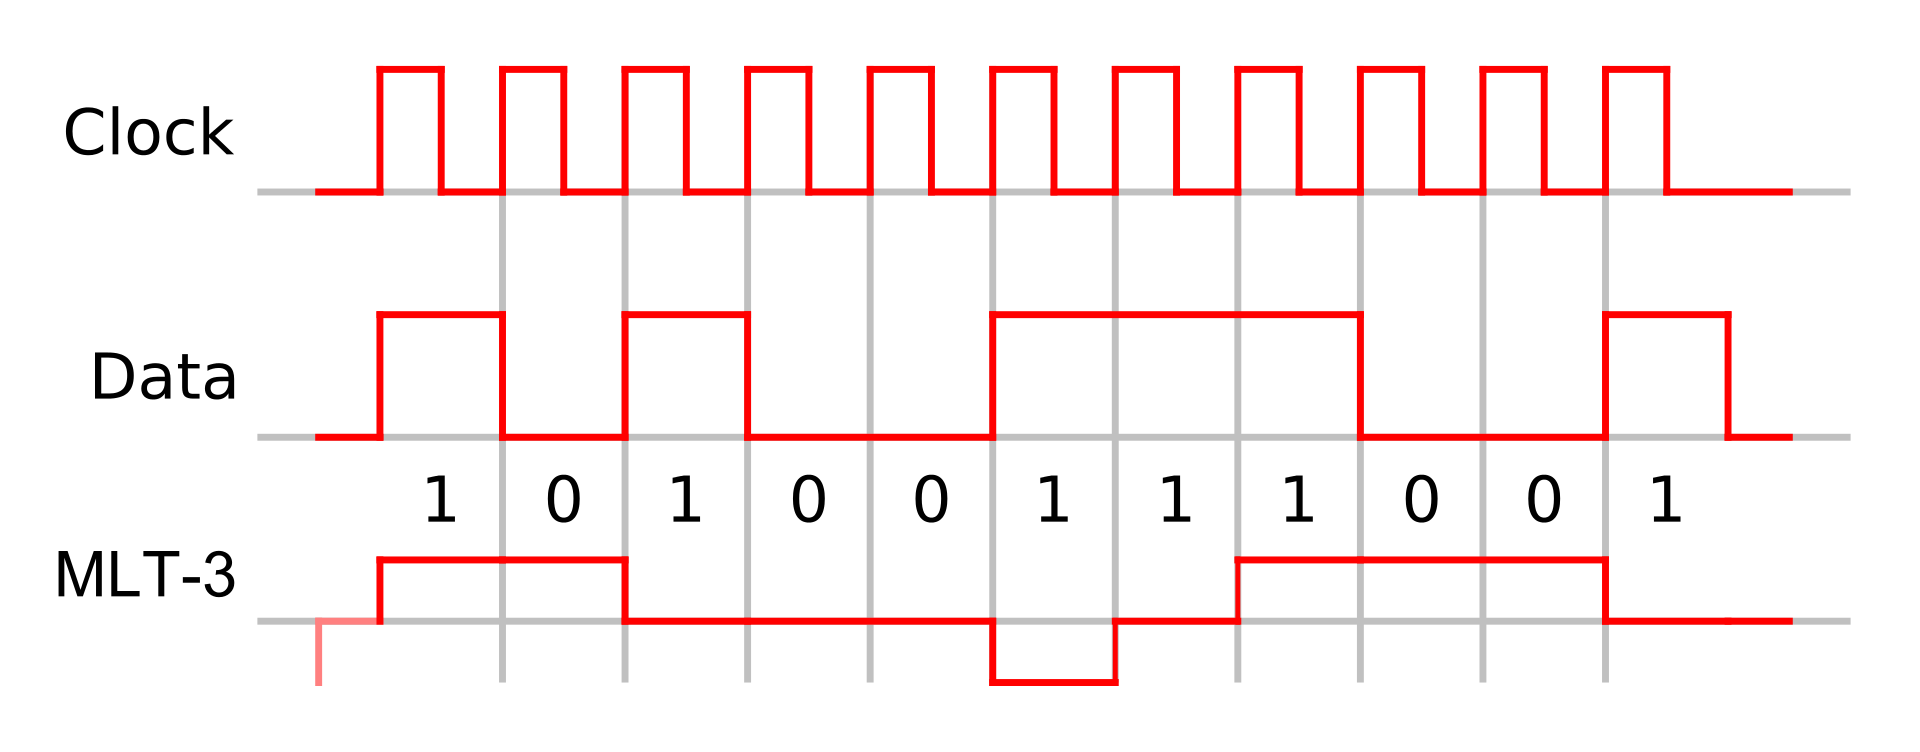
\includegraphics[width=\textwidth]{MLT3encoding.png}
    \caption{Clock dient zur Markierung der Übergangszeitpunkte}
\end{figure}
\end{center}
\break

Die Spannung ändert sich wie bereits erwähnt jedes Mal wenn eine logische Eins verabreitet wird. Diese Änderung variert folgender
Reihenfolge:

\begin{enumerate}
	\item Von 0 auf +
	\item Von + auf 0
	\item Von 0 auf -
	\item Von - auf 0
\end{enumerate}

Diese vier Schritte wiederholen sich jedes Mal bei einer logischen Eins in genau dieser Reihenfolge.

\section{Bedienanleitung}

\begin{center}
\begin{figure}[h]
    \centering
    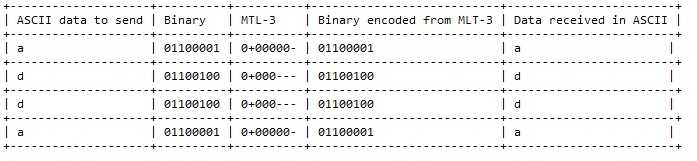
\includegraphics[width=16cm]{output2.png}
    \caption{Ausgabe mit Aufruf .mlt3send dsad}
\end{figure}
\end{center}

Durch den bloßen Aufruf des Programms, wie zum Beispiel \underline{./mlt3send}. Wird der Prozess ohne speziellen Funktionen
gestartet. Eine zufällige Einzahl von ASCII-Zeichen wird zufällig oft (zwischen 1 und 127 mal) auf der Konsole als Tabelle formatiert ausgegben.
Die Tabelle zeigt das gewählte ASCII Zeichen, die binäre Kodierung dazu, dann den MLT-3 Übertrag, dann diesen als binär wieder zurückübersetzt
und schließlich in der letzten Spalte, das dekodeirte ASCII-Zeichen wieder. (Abb. 2)

Wenn mann beim Aufruf den Programms, wie zum Beispiel  \underline{./mlt3send dsad} eingibt. Werden die einzelnen Zeichen hinter dem Programmnamen
überprüft, ob sie in ASCII enthalten sind und im positiven Fall, wird das Programm genau wie bei einem einfachen Aufruf gestartet. Nur diesmal werden
bloß die ASCII-Zeichen, welche hinter dem Programmnamen stehen zufällig oft (zwischen 1 und 127 mal) übertragen. \\

\begin{itemize}
	\item \underline{Eingabe:} ./mlt3send dsad
	\item \underline{Ausgabe:} [Siehe Abb. 2]\\
\end{itemize}

\begin{center}
\begin{figure}[h]
    \centering
    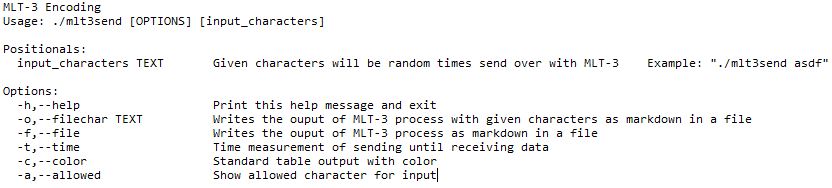
\includegraphics[width=16cm]{climenu.png}
    \caption{Hilfe des Programms in der Kommandozeile}
\end{figure}
\end{center}

Option \textbf{-h,--help}:\\
Zeigt die Hilfe für das Programm an, liefert das Menü wie in Abb. 3 zurück.
\begin{itemize}
	\item \underline{Eingabe:} ./mlt3send -h
	\item \underline{Ausgabe:} [Siehe Abb. 3]\\
\end{itemize}

Option \textbf{-o,--filechar TEXT}:\\
Startet das Programm und schreibt das Ergebnis als markdown in eine Datei, Speicherort der Datei wird nach Aufruf auf der Konsole ausgegeben.
Erwartet ASCII kodierbare Character als eingabe.
Beispiel: 
\begin{itemize}
	\item \underline{Eingabe:} ./mlt3send -o asdf
	\item \underline{Ausgabe:}

[NOTE]\\
The result is saved to the location: /home/maurice/Desktop/mlt3.mkd\\
It is formated as markdown.\\
\end{itemize}

Flag \textbf{-f,--file}:\\
Startet das Programm mit zufällig gewählten ASCII-Zeichen und schreibt sie als mardown in eine Datei, Speicherort der Datei wird nach Aufruf auf der Konsole ausgegeben.
Beispiel: 
\begin{itemize}
	\item \underline{Eingabe:} ./mlt3send -f
	\item \underline{Ausgabe:}

[NOTE]\\
The result is saved to the location: /home/maurice/Desktop/mlt3.mkd\\
It is formated as markdown.\\
\end{itemize}

Flag \textbf{-t,--time}:\\
Startet das Programm und gibt das Ergebnis auf der Konsole aus. Zusätzlich wird am Ende die gemessene Zeit in Nano und Mikrosekunden ausgegeben. Der Grund für die beiden
Einheiten ist, dass manchmal, wenn zufällig und ein Zeichen übertragen wird, oder der Computer sehr schnell ist, auf dem das Programm ausgeführt wird, dies unter
einer Mikrosekunde passiert.

Die gemessene Zeit wird mit Start des Sende-Threads angefangen, und endet mit der Verarbeitung aller Daten durch den Empfängerthread. Die Ausgabe in die Konsole oder
das schreiben in eine Datei wird \underline{nicht} mitgemessen, jedoch die Erstellung der Tabelle für die weitere Ausgabe schon.

Beispiel: 
\begin{itemize}
	\item \underline{Eingabe:} ./mlt3send -t
	\item \underline{Ausgabe:}

(Tabelle mit den Werten wie in Abb. 2)\\
.\\
.\\
.\\
Elapsed time in nanoseconds  : 1058770 ns\\
Elapsed time in microseconds : 1058 µs\\
\end{itemize}

Flag \textbf{-c,--color}:\\
Startet das Programm normale mit zufällig gewählten ASCII Zeichen und gibt die Tabelle färbig aus.\\
\underline{Achtung:} kann je nach Terminal-Anwendung und Computer zu schlechter Performance bei der Ausgabe führen. Die Geschwindigkeit der Übertragung wird
allerdings nicht beeinflusst.

\begin{itemize}
	\item \underline{Eingabe:} ./mlt3send -c
	\item \underline{Ausgabe:} Tabelle wie in Abb. 2 nur farbig\\
\end{itemize}

Flag \textbf{-a,--allowed}:\\
Damit kann man alle erlaubten ASCII Zeichen für das Programm sich anzeigen lassen. Einige ASCII Zeichen wie zum Beispiel 1 - SOH (start of heading), in C++ nicht über die
Kommandozeile gewünscht verarbeitet werden kann. Alle Zahlen und Buchstaben und die meisten welche in ASCII enthalten sind, werden unterstützt.

\begin{itemize}
	\item \underline{Eingabe:} ./mlt3send -a
	\item \underline{Ausgabe:} Tabelle, wo auf der linken Seite Dezimal-Werte stehen und auf der rechten Seite die jeweiligen zugerhörigen ASCII Zeichen.\\
\end{itemize}

\section{Umsetzung}
Das Programm legt nach dem Parsen ein Objekt, einer selbst erstellten Klasse einer Thread-Safe Queue an. Anfangs war nicht sicher welchen Typ der queue unterstützen sollte,
demnach wurden templates verwendet. Die Implementierung der Thread-Safe Queue Klasse befindet sich im \underline{indlude} Verzeichnis in der Datei \underline{queue.h}. Sie
wurde im Header definiert, da die Verwendung von templates keine Aufteilung der Implementation in eine .cpp Datei zuließ.

Danach wird ein Thread \underline{sender} erstellt:
\begin{lstlisting}
thread sender{send_data_tf, random_tf(ref(main_table),
		     input_chars), ref(q), ref(main_table)};
\end{lstlisting}

Dieser Thread ruft eine Funktion:
\begin{lstlisting}
void send_data_tf(vector<int> data_to_send,
				Queue<string>& queue, Table& tab)
\end{lstlisting}

Diese Funktion bekommt einen vector vom Typ \underline{int}, eine Referenz zur vorhin angelegten Queue vom Typ \underline{string} und eine Referenz zu einer vorhin
angelegten Tabelle aus der externen Bibliothek \underline{tabulator.h}. Die Funktion liefert nichts zurück, der vector enthält die zufällig erstellten ASCII-Zeichen in Dezimaldarstellung.
Diese integer, welche einen Wert zwischen 33 und 127 haben können (alle zulässigen ASCII-Zeichen), werden in der Funktion zuerst auf einen Hilfs-vector in ihrer binären Darstellung
gepusht und dann mittels einer Funktion als MLT-3 kodiert auf den Queue als \underline{string} gepusht. 

Die Funktion dazu:
\begin{lstlisting}
string convert_to_mlt3(bitset<8> binary_block)
\end{lstlisting}

Diese liefert einen \underline{string} zurück und benötigt eine bitset mit 8 Stellen als Parameter. In der Funktion send\_data\_tf(...), wird diese Funktion hier für jedes Zeichen
einmal Aufgerufen. Der zurückgelieferte string, welcher zum Beispiel so aussehen kann: \underline{0+00---0}, wird auf die Queue gepusht.

Der Thread \underline{sender} benutzt um die Werte für den ersten Paramter Funktion send\_data\_tf(...) zu bekommen selbst auch eine Funktion:
\begin{lstlisting}
vector<int> random_tf(Table& tab, string allowed="")
\end{lstlisting}

Diese Funktion liefert den vector vom Typ \underline{int} zurück welcher in der Funktion send\_data\_tf(...) benötigt wird. Sie bekommt selbst eine Referanz auf die
Tabelle für die Ausgabe später mit und einen \underline{string} names "allowed". Dieser ist per default ein Leerstring. Falls dem Programm beim Start entsprechende Zeichen mitgeben
werden, wird nur aus dieser Zeichenmenge dann eine zufällige Anzahl davon in den Vektor eingefügt. Insgesamt können insgesamt Zeichen zwischen 1 und 127 mal in den Vector eingefügt
werden, dies hat keinen speziellen Grund, man könnte theoretisch das obere Limit an Zahlen auch bis zum maximalen vector-Größe Limit setzen. Jedoch wäre das nicht sinnvoll, da die Ausgabe
in der Kommandozeile sehr lange dauern würde und andere Probleme mit dem Speicher auftreten würden, bei Interesse sind dazu weiter unten Links. 

Die maximale vector Größe könnte man
wie folgt feststellen:
\begin{lstlisting}
std::vector<int> myvector;
std::cout << "max_size: " << myvector.max_size();

//Moegliche Ausgabe:

max_size: 1073741823
\end{lstlisting}


Nach diesem Prozess wird ein andere Thread gestartet:
\begin{lstlisting}
thread receiver{decode, ref(q), ref(main_table)};
\end{lstlisting}

Dieser Thread namens \underline{receiver}, ruft folgende Funktion auf:
\begin{lstlisting}
void decode(Queue<string>& queue, Table& tab)
\end{lstlisting}
Diese Funktion decode(...), liefert nichts zurück. Ihre Aufgabe ist, den Queue in einer while-Schleife abzuarbeiten, jedes Element zuerst von MLT-3 mittels einer Hilfsfunktion 
ins binäre zurück, und dann schließlich als ASCII-Zeichen zu übersetzen.

Die Hilfsfunktion:
\begin{lstlisting}
decrypt_from_mlt3(string mlt3_data, Table& tab, int table_col_cnt)
\end{lstlisting}

Sie wird für jedes Element im Qeue einmal aufgerufen, der Aufruf geschieht in der vorherig dargestellten Funktion \underline{decode(...)}. Sie bekommt beim Aufruf die Referent auf die
Tabelle von der Bibliothek \underline{tabulator.h} mit, damit sie die Werte in die jeweillige Spalte und Reihe eintragen kann, da das Element nach der Abarbeitung vom Queue gelöscht wird.
Weiters bekommt die Funktion natürlich einen \underline{string} names \underline{mlt\_data} mit, welchen sie zuerst ins binäre, und dann mittels einem \underline{sstringstream} aus 
der standard-Bibiothek, in eine bitset mit acht Stellen unwandelt und schließlich zurück in eine ASCII-Zeichen.


\subsection{Verwendete Externe Klassen}
\begin{itemize}
	\item \underline{rang-library:} für die farbige Ausgabe der Tabelle
	\item \underline{CLI11-library:} für die Verarbeitung von Eingabe und Options- und Funktionsargumenten
	\item \underline{spdlog-library:} für das Logging
	\item \underline{tabulate-library:} für die Formatierung der Ausgabe als Tabelle
\end{itemize}


\section{Quellen}

\begin{itemize}
	\item https://de.wikipedia.org/wiki/MLT-3-Code
	\item https://de.wikipedia.org/wiki/Ternäres\_Signal
	\item https://www.cplusplus.com/reference/vector/vector/max\_size/
	\item Link zu Limit von vektoren: https://stackoverflow.com/questions/32316346/limit-on-vectors-in-c
	\item Folie 21. "Encoding and Decoding" aus dem NVS Unterricht
\end{itemize}

\textbf{Alle benutzen Bilder sind frei für akademische Zwecke zu benutzen oder das Urheberrecht liegt beim Verfasser (Maurice Putz)}

\end{document}